\documentclass[a4paper,oneside,12pt]{article}

\usepackage[top=3.0cm,bottom=2.0cm,left=2.9cm,right=2.9cm]{geometry}
\usepackage[portuges]{babel}
\usepackage{amsmath,amsfonts,amssymb}
\usepackage{graphicx,color}
\usepackage{enumerate}
\usepackage{amsmath}
\usepackage{mathtools}
\usepackage{color}
\usepackage{pdfpages}

\begin{document}

\bfseries
\noindent
Universidade Federal do Rio Grande do Norte \\
Programa de P\'os-Gradua\c{c}\~ao em Engenharia El\'etrica e de Computa\c{c}\~ao \\
Redes Neurais (EEC1505) \\
Prof. Adri\~ao Duarte Doria Neto \\
Alunos: Jos\'e Lenival Gomes de Fran\c{c}a, Raphael Diego Comesanha e Silva, Danilo de Santana Pena.
\mdseries

\begin{center}
Lista 3 Exerc\'icios
\end{center}

\begin{enumerate}[1.]
\item A representa\c{c}\~ao de uma determinada mensagem digital tern\'aria, isto \'e formada por tr\^es bits, forma um cubo cujos v\'ertices correspondem a mesma representa\c{c}\~ao digital. Supondo que ao transmitirmos esta mensagem a mesma seja contaminada por ru\'ido formando em torno de cada v\'ertice uma nuvem esf\'erica de valores aleat\'orios. O raio da esfera corresponde ao desvio padr\~ao do sinal de ru\'ido. Solucione o problema usando m\'aquinas de vetor de suporte linear. Compare com a solu\c{c}\~ao obtida na lista 2 onde foi usada uma rede de perceptron de Rosemblat com uma camada para atuar como classificador/decodificador. Para solu\c{c}\~ao do problema defina antes um conjunto de treinamento e um conjunto de valida\c{c}\~ao. \\

RESOLU\c{C}\~AO: \\

... \\

\item Implemente a RBF considerando os algoritmos de treinamento para as tr\^{e}s situa\c{c}\~oes: (a) centros fixos e escolhidos aleatoriamente, (b) centros escolhidos atrav\'es da sele\c{c}\~ao auto-supervisionada (algoritmo K-means) , (c) centros escolhidos atrav\'es da sele\c{c}\~ao supervisionada, para as tr\^es quest\~oes abaixo: \\

\begin{enumerate}[a)]
\item A fun\c{c}\~ao l\'ogica $f(x_{1}, x_{2}, x_{3}) = x_{1} \oplus x_{2} \oplus x_{3}$

\item \begin{equation*}
f(x) = \left[ \frac{sin(\pi ||x||)}{\pi ||x||} \right] \text{, } x = \begin{bmatrix}
x_{1} \\
x_{2}
\end{bmatrix} \text{, } |x_{1}| \leq 10 \text{ e } |x_{2}| \leq 10
\end{equation*}

\item $f(x) = x_{1}^{2} + x_{2}^{2} - 2 x_{1} x_{2} + x_{1} + x_{2} - 1$, $|x_{1}| \leq 10$, $|x_{2}| \leq 10$
\end{enumerate}

RESOLU\c{C}\~AO: \\

As alternativas $a)$ e $c)$ possuiram erro igual a $0$. Na alternativa $b)$ n\~ao conseguiu-se bons resultados utilizando a $toolbox$, pois a sa\'ida da rede resulta em valor $NaN$.

Segue o c\'odigo utilizando a \emph{toolbox} do MATLAB:

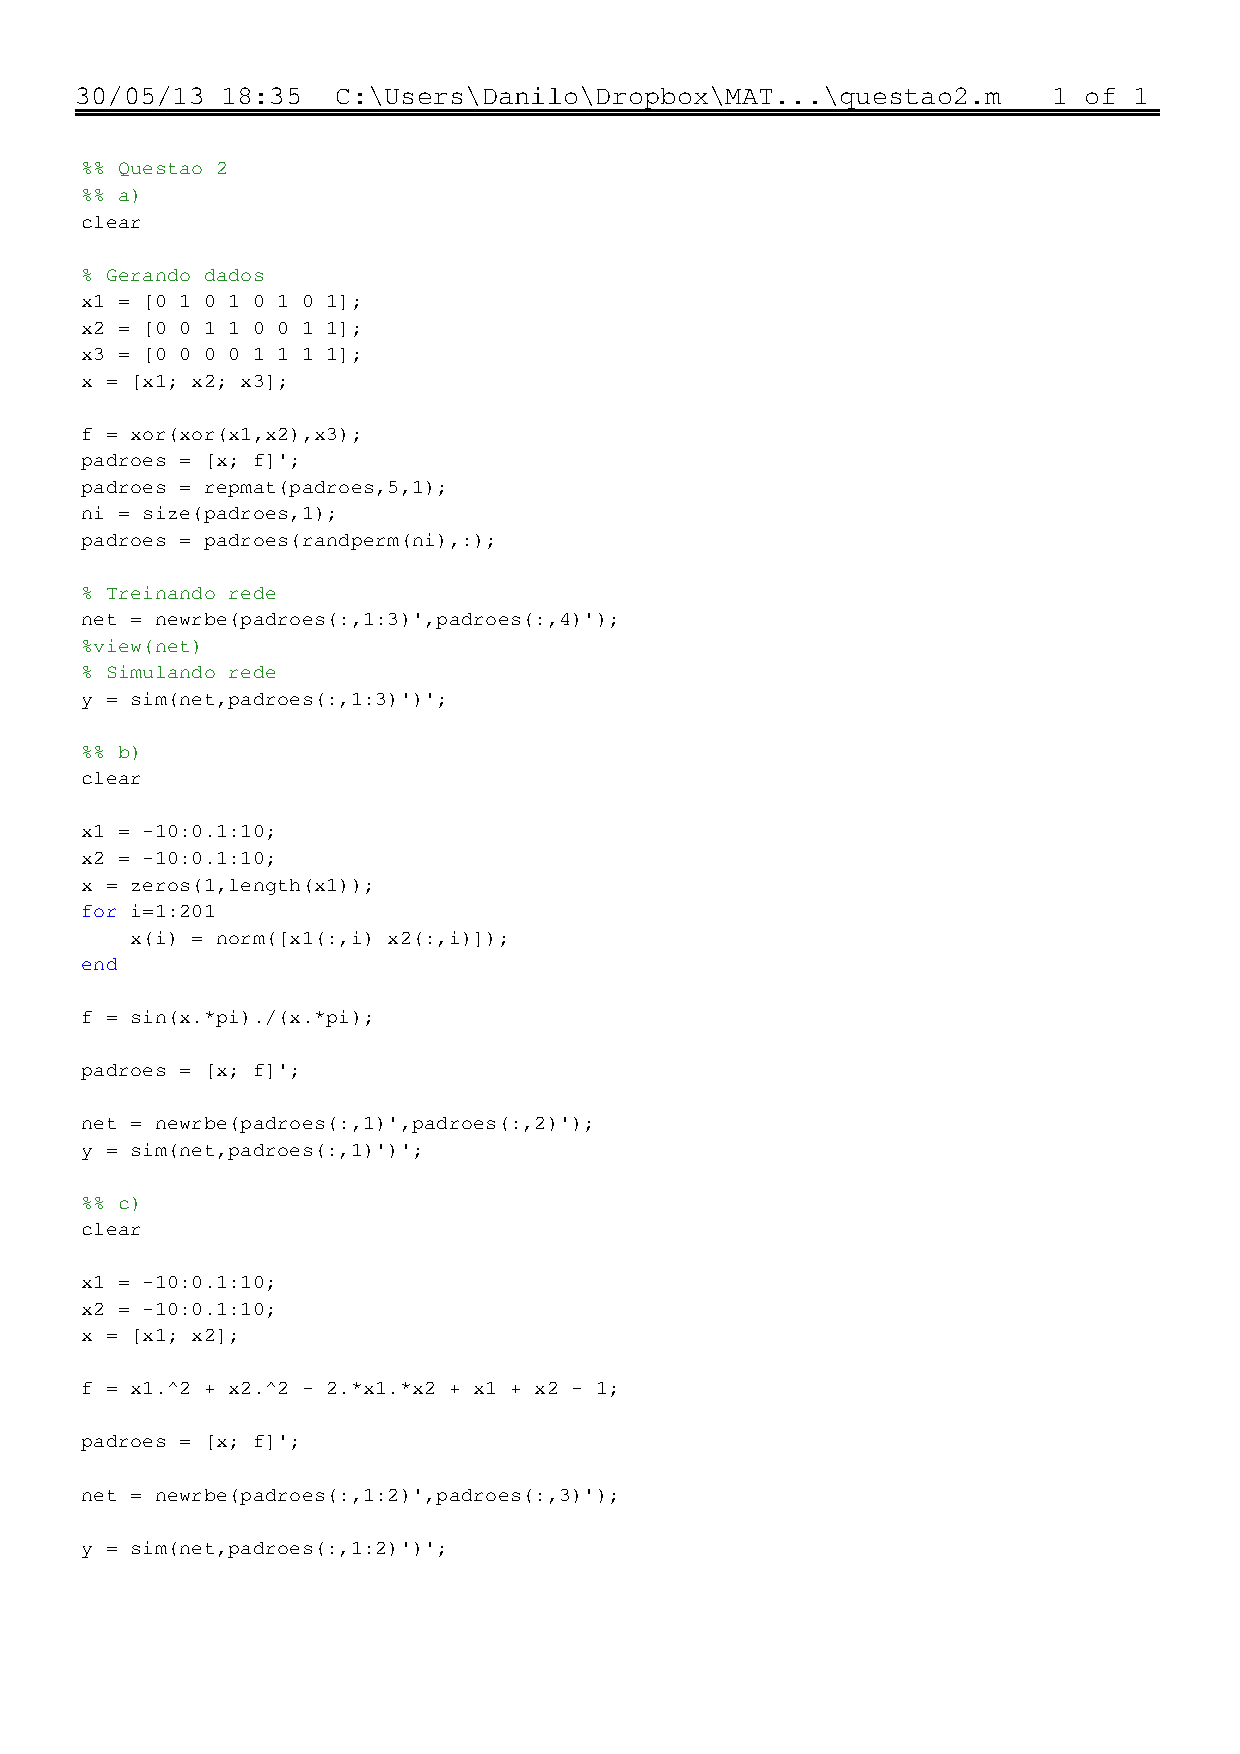
\includepdf[pages=-]{q2.pdf}

\item Considere o problema de classifica\c{c}\~ao de padr\~oes constitu\'ido neste caso de 12 padr\~oes. A distribui\c{c}\~ao dos padr\~oes tem como base um quadrado centrado no ponto (0.5,0.5) e lados iguais a 1. Os pontos (0.5,0.5), (1.0,0.5), (0.5,1.) e (0.0, 0.5) s\~ao centros de quatro semic\'irculos que se interceptam no interior do quadrado originando quatro classes e outras oito classes nas regi\~oes de n\~ao interse\c{c}\~ao. Ap\'os gerar aleatoriamente dados que venham formar estas distribui\c{c}\~oes de dados, selecione um conjunto de treinamento e um conjunto de valida\c{c}\~ao. Solucione o problema usando RBF, SVM e M\'aquina de Comit\^e. Verifique o desempenho do classificador usando o conjunto de valida\c{c}\~ao e calculando a matriz de confus\~ao e compare com o obtido na lista anterior usando MLP. \\

RESOLU\c{C}\~AO: \\

\item Utilize uma rede NARX, no caso uma rede neural perceptron de m\'ultiplas camadas com realimenta\c{c}\~ao global, para fazer a predi\c{c}\~ao de um passo, at\'e predi\c{c}\~ao de tr\^es passos da s\'erie temporal $x(n) = 1 + cos(n + cos 2 (n))$. Avalie o desempenho mostrando para cada caso os erros de predi\c{c}\~ao. \\

RESOLU\c{C}\~AO: \\

\item Implemente uma rede de Hopfield, para reconhecer as letras AFC. (Para cada letra forme uma matriz bin\'aria de pixel). Verifique o desempenho com as letras sendo apresentadas de forma ruidosa. \\

RESOLU\c{C}\~AO: \\

\item Dado o modelo n\~ao linear de espa\c{c}o de estado abaixo, obtenha o modelo de espa\c{c}o de estados linearizado para ser utilizado no algoritmo EKF. \\

\begin{equation*}
x(n+1) = f(n, x(n)) + v_{1}(n)
\end{equation*}

\begin{equation*}
y(n) = c(n,x(n)) + v_{2}(n)
\end{equation*}

\begin{equation*}
f(n, x(n)) = \begin{bmatrix}
x_{1}(n) + x_{2}^{2}(n) \\
nx_{1}(n) - x_{1}(n)x_{2}(n)
\end{bmatrix}
\end{equation*}

\begin{equation*}
c(n, x(n)) = x_{1}(n)x_{2}^{2}(n) + v_{2}(n)
\end{equation*}

RESOLU\c{C}\~AO: \\

\item Um problema interessante para testar a capacidade de uma rede neural atuar como classificado de padr\~oes \'e o problema das duas espirais intercaladas. Gere os exemplos de treinamento usando as seguintes equa\c{c}\~oes: \\
para espiral 1 $x = \frac{\theta}{4} cos(\theta)$ , $y = \frac{\theta}{4} sen(\theta)$ , $\theta \geq 0$ \\
para espiral 2 $x = (\frac{\theta}{4} + 0.8) cos(\theta)$ , $y = (\frac{\theta}{4} + 0.8) sen(\theta)$ , $\theta \geq 0$ \\
fazendo $\theta$ assumir 51 igualmente espa\c{c}ados valores entre 0 e 20 radianos. Utilize uma rede competitiva e em seguida uma rede SOM para atuar como classificador auto-supervisionado, isto \'e, a espiral 1 sendo uma classe e espiral 2 sendo outra classe. Para comparar as regi\~oes de decis\~oes formadas pela rede , gere uma grade uniforme com 100 x 100 exemplos de teste em um quadrado [-5,5]. Esboce os pontos classificados pela rede. \\

RESOLU\c{C}\~AO: \\

Foram implementados o algoritmo competitivo e o algoritmo SOM, como segue abaixo junto com o resultado:

\begin{figure}[h]
\centering
\includegraphics[width=0.8\textwidth]{q7.png}
\caption{Resultado da rede SOM para a espiral.}
\label{fig:q7}
\end{figure}

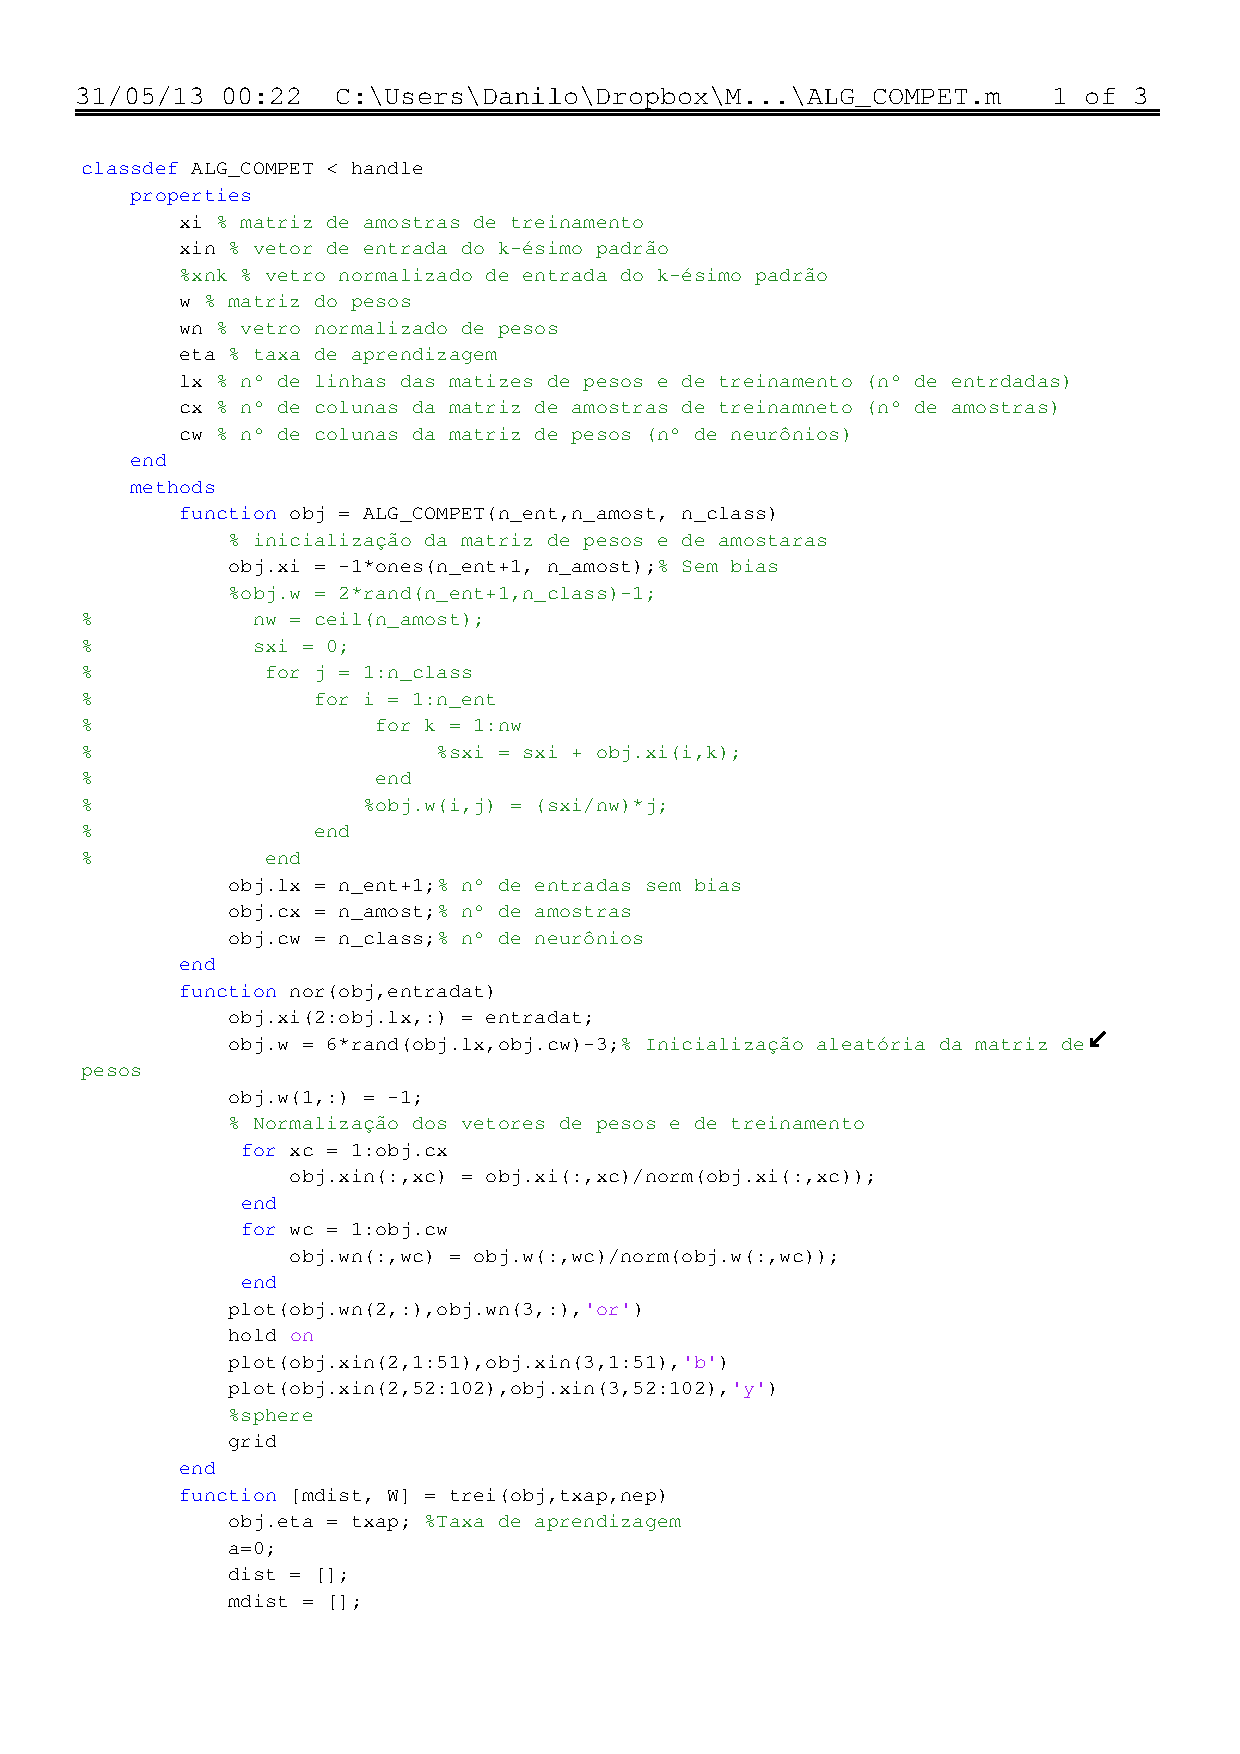
\includepdf[pages=-]{q7_1.pdf}

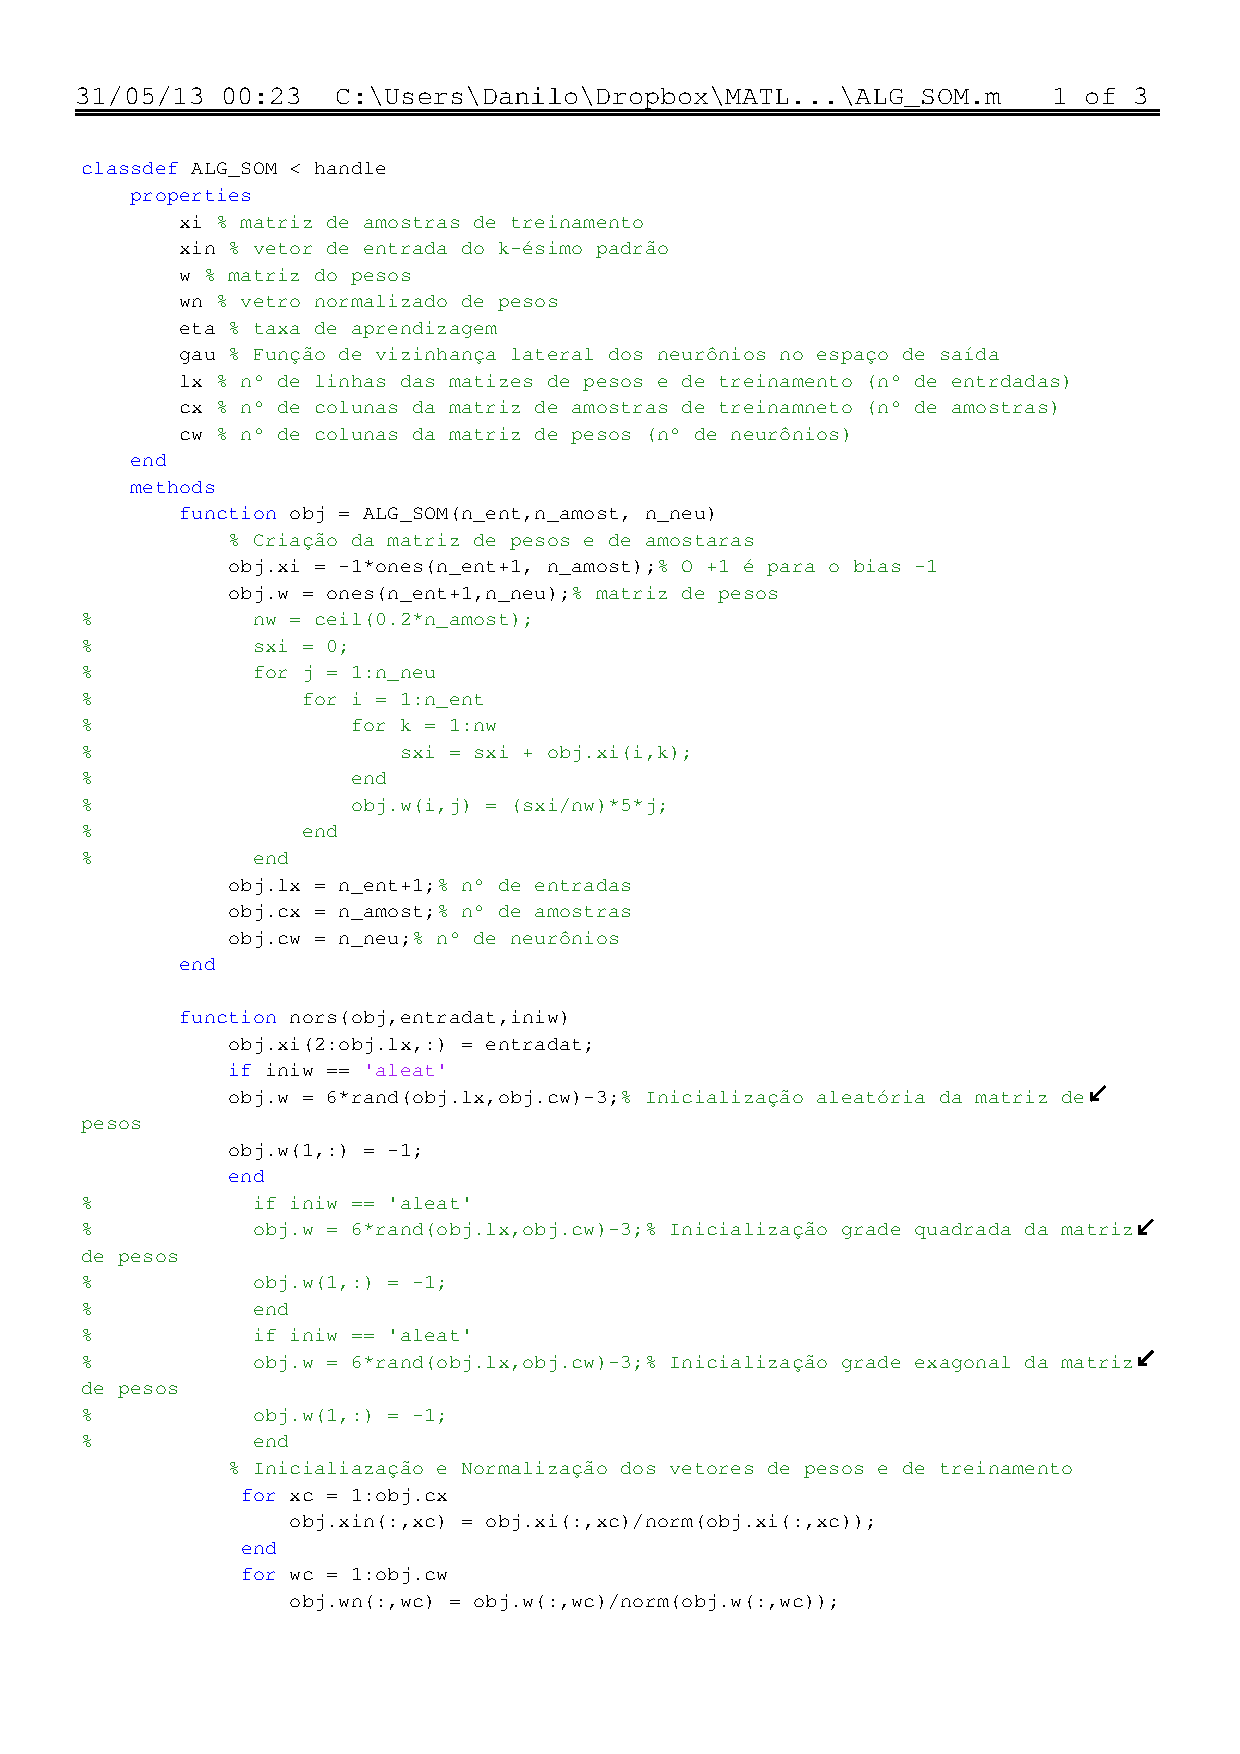
\includepdf[pages=-]{q7_2.pdf}

\item Considere a distribui\c{c}\~ao dos padr\~oes que tem como base em um c\'irculo com raio igual a 0.25 centrado origem. Os pontos +1 e -1 de cada eixo s\~ao centros de quatro semic\'irculos que se interceptam no interior a as regi\~oes que excluem o c\'irculo de raio igual a 0.25 do quadrado originando quatro classes. Gere aleatoriamente os dados que venham formar estas distribui\c{c}\~oes de dados. Utilize a rede SOM de modo a quantizar atrav\'es da distribui\c{c}\~ao de neur\^onios a distribui\c{c}\~ao dos dados. \\

RESOLU\c{C}\~AO: \\

Foi feito a gera\c{c}\~ao dos dados atrav\'es da equa\c{c}\~ao do c\'irculo:

\begin{equation*}
x = \sqrt{r^{2} - (y - y_{0})^{2}} + x_{0}
\end{equation*}

\begin{equation*}
y = \sqrt{r^{2} - (x - x_{0})^{2}} + y_{0}
\end{equation*}

A classifica\c{c}\~ao dos dados foi feito atrav\'es de um vetor $[QX QY H V]$, em que para cada ponto gerado $QX$ representa um dos dois quadrantes no eixo $X$, podendo assim assumir o valor $0$ ou $1$, o equivalente ocorre para $QY$ no eixo $Y$, $H$ representa se o ponto gerado encontra-se dentro de um semi-c\'irculo horizontal e $V$ para um semi-c\'irculo vertical. Com este vetor \'e poss\'ivel classificar o ponto gerado, visto que se o ponto estiver com valores de $H$ e $V$ iguais a $1$ significa que o ponto encontra-se dentro de dois semi-c\'irculos simultaneamente, ou seja, na regi\~ao de interesse. Os valores de $QX$ e $QY$ descrevem em quais das quatro regi\~oes os pontos se encontram.

\begin{figure}
\centering
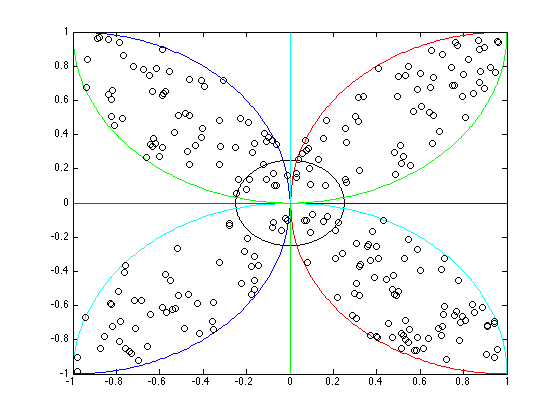
\includegraphics[width=0.8\textwidth]{q8_1.png}
\caption{Desenho das regioes de interesse.}
\label{fig:q8_1}
\end{figure}

A rede foi treinada utilizando a \emph{toolbox} do MATLAB, com o m\'etodo $newsom$, com uma arquitetura 10x10 uniformimente distribuida. Com 500 pontos gerados e 200 itera\c{c}\~oes, tem-se:

\begin{figure}
\centering
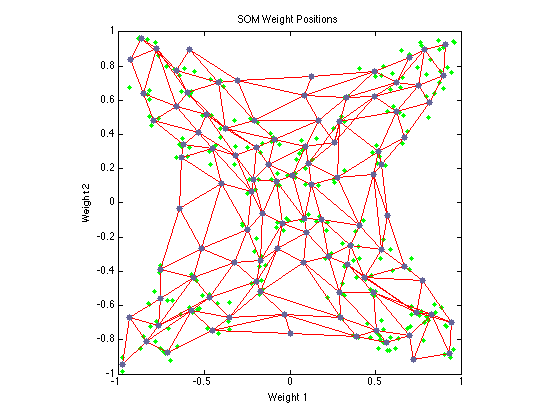
\includegraphics[width=0.8\textwidth]{q8_2.png}
\caption{Resultado da rede.}
\label{fig:q8_2}
\end{figure}

\begin{figure}
\centering
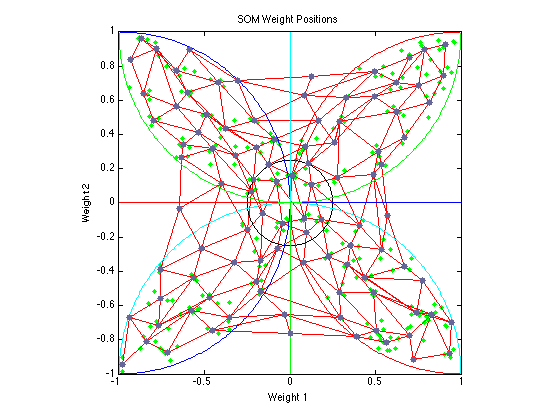
\includegraphics[width=0.8\textwidth]{q8_3.png}
\caption{Resultado da rede com as regioes.}
\label{fig:q8_3}
\end{figure}

\newpage

\item Pesquise e apresente o formalismo do algoritmo K-means por lote. \\ 

RESOLU\c{C}\~AO: \\

\item Pesquise e apresente o formalismo do algoritmo SOM por lote. \\

RESOLU\c{C}\~AO: \\


\end{enumerate}

\newpage

\begin{center}
Trabalhos
\end{center}

\begin{enumerate}[1.]
\item Pesquise e apresente um trabalho sobre a reconstru\c{c}\~ao tridimensional usando a rede SOM e a rede Neuro-GAS. \\

\item Pesquise e apresente um trabalho sobre Neurofuzzy.
\end{enumerate}

Data de entrega: 23/05/2013 \\

A entrega e apresenta\c{c}\~ao dos trabalhos correspondem a um processo de avalia\c{c}\~ao. Portanto a presen\c{c}a \'e obrigat\'orio. \\

Os trabalhos e a lista podem ser feito em grupo de at\'e tr\^es componentes. \\

Na apresenta\c{c}\~ao os componentes ser\~ao submetidos a questionamentos sobre a solu\c{c}\~ao da lista e o desenvolvimento dos trabalhos. \\

\newpage

\begin{center}
Desenvolvimento da Pesquisa
\end{center}

...

\end{document}